\chapter{Úvod}

Možnosti pripojenia rôznych periférií k zariadeniu sú v dnešnej dobe rozsiahle. Aj napriek tomu, že technológia každým dňom napreduje a svet sa uberá viac bezdrôtovým smerom, je USB stále najrozšírenejší sériový spôsob prenášania dát. Už z názvu \uv{Universal Serial Bus} je jasné, že rozpätie zariadení, ktoré možno k tejto zbernici pripojiť je obrovské. Práve preto je USB protokol jeden z najkomplexnejších protokolov ktoré sa využívajú na komunikáciu.

V tejto práci sa pozrieme na užšiu podmnožinu USB protokolu a na komunikáciu s dopredu vybratými perifériami, konkrétne myšou, klávesnicou a joystickom.

\section{USB}
vysvetlenie zakladnych pojmov spojenych USB: historia, usb port/conector, plug and play(https://docs.microsoft.com/en-us/windows-hardware/drivers/kernel/introduction-to-plug-and-play), host-master, low/full/high speed zariadenia

\section{Existujúce aplikácie}

Momentálne existuje niekoľko známych aplikácií ktoré slúžia na analýzu USB paketov. V tejto kapitole si ich zopár ukážeme, pričom mnohé z nich nám poslúžili ako inšpirácia pri ppísaní našej práce a riešení konkrétnych problémov na ktoré sa pozrieme v nasledujúcich kapitolách. 

Je nutné upozorniť, že väčšina dnešných analyzátorov sú platené aplikácie, prípadne majú odomknuté len základné vlastnosti s možnosťou dokúpenia si plnej verzie. Práve preto pri ich prípadnom porovnávaní budeme brať do úvahy len funkcionalitu, ktorá je dostupná zadarmo.

\subsection*{Wireshark}

Pravdepodobne najznámejšia third-party aplikácia na analýzu paketov. Jeho funkcionalita je veľmi rozsiahla, a vzhľadom na to, že sa jedná o open-source projekt, neustále rastie. Zameriava sa hlavne na analýzu sieťových paketov. Napriek tomu podporuje spoluprácu s rôznymi inými sniffermi. Jeden z takýchto snifferov je USBPcap ktorý zachytáva USB komunikáciu, a tak nie je prekvapivé, že Wireshark podporuje analýzu paketov aj nad touto zbernicou. 

Vzhľadom na obľúbenosť a rozsiahlosť programu, nám Wireshark poslúžil ako referenčná aplikácia, z ktorej sme čerpali celkovú inšpiráciu na funkcie, ktoré by mal bežný analyzátor paketov spĺňať. Medzi tie úplne základné patrí napríklad hexdump dát nad ktorými prebieha analýza, ale napríklad aj spôsob vyobrazenia rôznych deskriptorov, ktoré je riešené cez stromovú štruktúru. Medzi viac špecifické funkcie ktoré sme neskôr implementovali aj v našom programe patrí napríklad detailnejšie vyobrazenie jednotlivých bytov a ich význam, ako je možné vidieť nižšie na obrázku~\ref{obr:uvod:byte_detail_foto}. Túto vlastnosť aj napriek jej využitiu mnohé konkurenčné aplikácie postrádajú.

Jeho výhoda je hlavne v tom, že podporuje širokú škálu deskriptorov a plná verzia programu je dostupná úplne zadarmo. Z pohľadu užívateľa je až prekvapivé, že aj napriek rozsiahlosti programu je aplikácia veľmi user-friendly orientovaná a dopĺňa ju veľmi intuitívne užívateľské rozhranie.

\begin{figure}
	\centering
	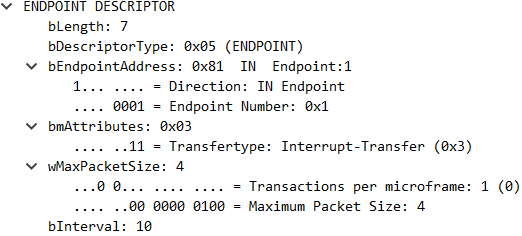
\includegraphics[width=\textwidth]{img/uvod_byte_detail}
	\caption{Ukážka vyobrazenia jednotlivých bytov.}
	\label{obr:uvod:byte_detail_foto}
\end{figure}

\subsection*{Device Monitoring Studio}

Plná verzia aplikácie je platená. Verzia zadarmo ponúka analýzu sieťových a USB paketov, tak ako aj analýzu komunikácie prebiehajúcej cez sériový port. 

Ako prvé na aplikácii zaujme spôsob zvolenia si zariadenia s ktorým bude sledovaná komunikácia. Je implementovaný štýlom stromovej štruktúry ako je ukázané na obrázku~\ref{obr:uvod:treeview_foto} nižšie. Už základná verzia programu poskytuje veľmi rosiahlu funkcionalitu. Používateľovi je umožnené posielať zariadeniu požiadavky definované v USB špecifikácii(ODKAZ). Aplikácia taktiež zobrazuje sémantickú analýzu niektorých HID zariadení, ale nie v práve najlepšej podobe. 

Na základe výstupu sa dá povedať, že sémantická analýza je naimplementovaná skôr obecne a pri niektorých položkách je namiesto ich významu napísané \uv{Unknown}. Taktiež nie je veľmi jasné odkiaľ sa dané hodnoty berú, keďže k nim chýba ich dátová reprezentácia. Medzi zachytenými paketami sa prvotne nezobrazujú tie, ktoré označujú nakonfigurovanie daného zariadenia (je nutné ho odpojiť a znova napojiť počas monitorovania). Užívateľské rozhranie je veľmi chaotické a chvíľu trvá, kým človek nájde čo i len základné informácie ako napríklad hlavičky ku jednotlivým paketom.  Nepoteší ani fakt, že verzia zadarmo nedovoľuje monitorovanie dlhšie ako 10 minút a maximálny počet monitorovaní za jeden deň je taktiež 10.

\newpage

\begin{figure}[!htb]
	\centering
	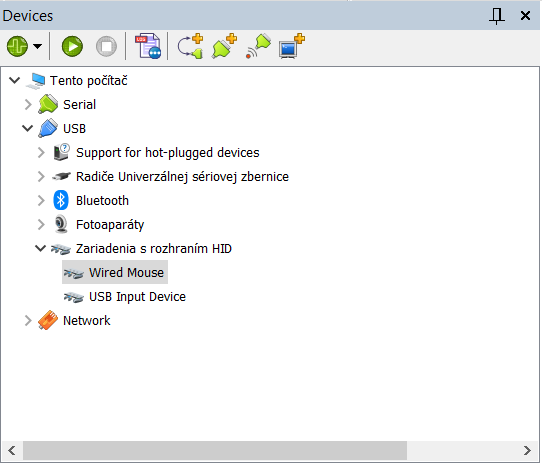
\includegraphics[width=\textwidth]{img/uvod_treeview}
	\caption{Ukážka stromovej štruktúry na zvolenie si zariadenia s ktorým bude zachytávaná komunikácia.}
	\label{obr:uvod:treeview_foto}
\end{figure}

\section{Požadované funkcie}
Na základe minulých príkladov už existujúcich aplikácií sme si mohli všimnúť, že všetky obsahujú niekoľko základných funkcií, ktoré by mal obsahovať každý analyzátor. V tejto sekcii zhrnieme funkcie, ktoré sme si zvolili pre našu aplikáciu. Zo základných funkcií sme si vybrali tie, ktoré považujeme za absolútne nevyhnutné pre každý analyzátor. Následne sme sa niekoľko z nich pokúsili akýmsi spôsobom vylepšiť tak, aby maximalizovali ich využiteľnosť a zároveň čo najlepšie zlepšovali prácu s aplikáciou jej užívateľovi. Zároveň ich dopĺňame o pokročilejšie funkcie z ktorých sú niektoré viac špecificky zamerané.

\subsubsection*{Základné}

Výsledná aplikácia by teda mala splňovať nasledujúce zákadné požiadavky:

\begin{enumerate}[label=\textbf{P\arabic*}]
	\item Mala by byť schopná analyzovať USB pakety zachytené v \textbf{pcap} formáte pomocou \textbf{USBPcap} snifferu.
	\item Mala by podporovať sémantickú analýzu pre všetky základné USB descriptory spomenuté v USB 2.0 dokumentácii(ODKAZ kapitola 9.6) (ako napríklad \textit{Device descriptor}, \textit{Interface descriptor}, \textit{Endpoint descriptor},...)
	\item Mala by vedieť rozumne zobraziť dáta ktoré \textbf{USBPcap} zachytí a uloží. Pod pojmom rozumne myslíme spôsob zobrazenia pomocou hexdumpu.
	\item Mala by na prvý pohľad jasne zobraziť základné informácie o každom analyzovanom pakete (ako napr. dĺžka paketu, typ prenosu, ...) a pri bližšom skúmaní jednotlivých paketov detailnejšie zobraziť celú jeho hlavičku.
	\item Detailnejšie informácie o pakete budú zobrazované na základe interakcie užívateľa s aplikáciou.
\end{enumerate}

\subsubsection*{Pokročilejšie}

Zároveň sme aplikáciu doplnili o niekoľko pokročilejších a špecificky zameraných požiadaviek:

\begin{enumerate}[label=\textbf{P\arabic*},resume]
	\item Mala by určitým spôsobom uľahčiť používateľovi orientáciu v hexdumpe.
	\item Mala by byť schopná rozparsovať \textbf{HID Report Descriptor} takým štýlom, aby bolo neskôr možné sématnicky reprezentovať input určitých HID zariadení
	\item Mala by byť schopná vhodným spôsobom vizuálne zobraziť sémantický význam dát posielaných danou podmnožinou HID zariadení do ktorej patrí myš, klávesnica a joystick.
	\item V miestach kde to dáva zmysel, by aplikácia mala byť schopná zobrazovať význam dát až na úrovni jednotlivých bitov.
\end{enumerate}

\section{Ciele práce}
vytvorit aplikaciu
navrh musi byt dostatocne obecny aby sa dal rozsirit o dalsie USB protokoly
dostatocne obecny navrh pre lahke pridavanie novych HID zariadeni
prehladny interface







